\documentclass{beamer} 
\usetheme{default} 
\usecolortheme{albatross}
\setbeamercovered{transparent}
%\useoutertheme{umbcfootline}  


\usepackage[spanish]{babel}
%\usepackage[latin1]{inputenc}
\usepackage[utf8x]{inputenc}
\usepackage{hyperref}
\usepackage{color}



%\usepackage{multicol}




\title{Excepciones en java}

\author{Manuel J. Molino Milla \and Luis Molina Garzón}

\date{\today} %

\institute{IES Virgen del Carmen \and Departamento de Informática}




%\beamerdefaultoverlayspecification{<+->}

\begin{document}


\begin{frame}
  \titlepage
\end{frame}

\begin{frame}
    \frametitle{Logo}
\begin{figure}

\includegraphics[scale=1]{imagenes/logo.jpeg} 
\caption{Logo Java}
\end{figure}
\end{frame}

%\begin{frame}
 % \frametitle{Contenido}
 %\tableofcontents[pausesections]
%\end{frame}




\begin{frame}[fragile]
\frametitle{Introducción}
\begin{itemize}[<+->]
\item El momento de capturar un error es en tiempo de compilación.
\item Pero no todos los errores se pueden detectar en tiempo de compilación.
\item Por lo que deben manejarse en tiempo de ejecución.
\item Ejemplo de errores en tiempo de ejución:
\begin{enumerate}
\item Acceder a una posición inexisten de una colección.
\item Acceder a un fichero que no existe.
\item Operaciones aritméticas no viables.
\item \dots
\end{enumerate}
\item Una \emph{condicion excepcional} es un problema que evita la continuación del programa.
\item Todo lo que se puede haces es salir del contexto actual y relegar el problema a un contexto diferente.
\end{itemize}
\end{frame}

\begin{frame}[fragile]
\frametitle{Ejemplo}
\begin{small}
\begin{verbatim}
Aplicacion app = new Aplicacion();
//Intento de login
Usuario u = app.login("juan","ssW12!ñ");
//Si los datos son incorrectos:
if (u==null){
  System.out.println("Usuario y/o contraseña no valido");
}else{
  System.out.println("Login con exito");
  System.out.println("Nombre: "+u.getNombre());
  System.out.println("Email: "+u.getEmail());
\end{verbatim}
\end{small}
\pause
\begin{footnotesize}
\begin{itemize}[<+->]
\item Supongamos que el login se verifica en una base de datos.
\item En ese momento la BD esta caida.
\item ¿En qué parte del código se hace la conexión a la BD?
\item ¿Que valor tiene entonces el método login?
\item Probablemente u es null y se entiende entonces que las credenciales no son validas.
\item Lo correcto es dar un aviso que la BD esta caida y no decir que las credenciales de acceso  son erróneas.
\end{itemize}
\end{footnotesize}
\end{frame}

 
\begin{frame}[fragile]
\frametitle{Excepciones basicas}
\begin{itemize}[<+->]
\item Las excepciones son reguladas en una clase.
\item Quiere decir que lanzar una excepcion implica crear un objeto.
\item En primer lugar se crea el objeto excepción  de la misma forma que se crea un objeto en Java: en el monticulo, con \bf{new}
\item Después se detiene el cauce normal de ejecución.
\item Y se lanza la referencia al objeto de excepción desde el contexto actual.
\item Ahora el gestor de excepciones debe recuperarse del programa
\item Ejemplo: comprobar que una referencia no se haya inicializado y así evitar que se llama a un método no apropiado:
\end{itemize}
\pause
\begin{verbatim}
if (t == null) throw new NullPointerException();
\end{verbatim}
Esto lanza la excepción y posteriormente en algún sitio se gestionará.
\end{frame}

\begin{frame}[fragile]
\frametitle{Parámetro de las excepciones}
\begin{itemize}[<+->]
\item Cuando se crea el objeto excepción se asigna espacio en el montículo e invoca a un constructor.
\item Hay dos constructores:
\end{itemize}
\pause
\begin{verbatim}
if (t == null) throw new NullPointerException();
\end{verbatim}
\pause
\begin{verbatim}
if (t == null) throw new NullPointerException("t es null");
\end{verbatim}
\begin{itemize}[<+->]
\item El \emph{string} puede extraerse posteriormente usando varios métodos.
\item Además se puede lanzar cualquier tipo de objeto \alert{Throwable}
\end{itemize}
\end{frame}


\begin{frame}
\frametitle{Tipos de excepciones}
\begin{figure}
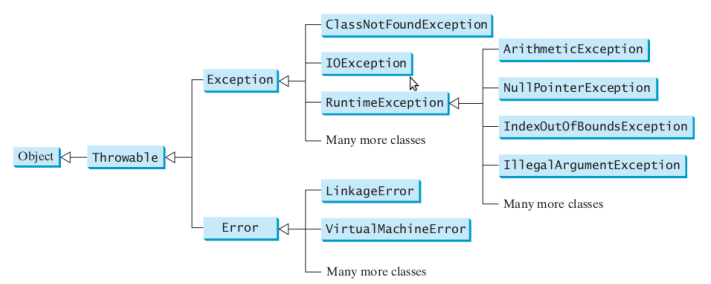
\includegraphics[scale=0.6]{imagenes/excepciones.png} 
\caption{Objetos Throwable}
\end{figure} 
\end{frame}

\begin{frame}
\frametitle{Tipos de excepciones}
\begin{itemize}[<+->]
\item \alert{Throwable} es la clase padre, cualquiera otra clase se hereda de esa clase.
\item Se pueden crear clases nuevas de excepciones pero deben heredar de la clase \alert{Exception} o de cualquier otra subclase.
\item Las excepciones se pueden clasificar en dos tipos:
\begin{description}
\item[Errores de sistema] son lanzadas por la JVM y representan la clase \alert{Error}, describen un error interno del sistema y raramene ocurren.
\item[Excepciones] representadas por la clase \alert{Exception} es el tipo básico que puede lanzarse desde cualquier método de las clases de la biblioteca estándar de Java y desde los métodos que uno elabore.
\end{description}
\end{itemize}
\end{frame}

%distinguir entre los dos tipos de excepcionesç

\begin{frame}[fragile]
\frametitle{Tipos de excepciones}
\begin{block}{Checked Exceptions}
Son escenarios donde podemos anticiparnos a esa situación excepcional y recuperarnos de ella, por ejemplo \emph{FileNotFoundException}
\end{block}
\pause
\begin{block}{Runtime Exception} 
Son causadas por malas prácticas de programación. Ejemplo intentar acceder a una posición no existente de una colección. Hay que comprobar previamente la longitud de la colección antes de intenta de acceder a algún elemento de la colección.
\end{block}
\end{frame}

\begin{frame}
\frametitle{Excepeciones no declarativas o RuntimeException}
\begin{itemize}[<+->]
\item Hay en Java excepciones que no hacen falta declararse y se lanzan automáticamente.
\item No hay que incluirlas en la especificación del método.
\item Estas excepciones se encuentran agrupadas en la clase \alert{RuntimeException}
\item Se les llama \alert{Excepeciones no declarativas}
\end{itemize}
%\begin{figure}
%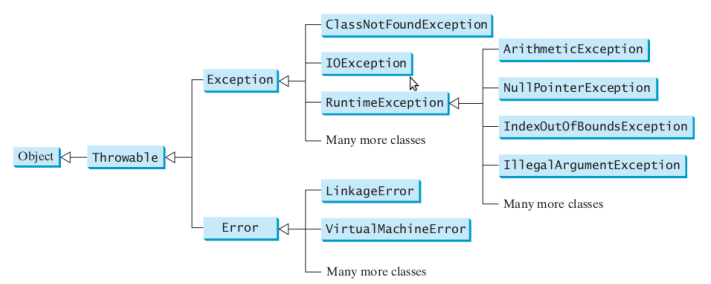
\includegraphics[scale=0.4]{imagenes/excepciones.png} 
%\caption{Objetos Throwable}
%\end{figure}
\end{frame}

\begin{frame}[fragile]
\frametitle{Ejemplo de RuntimeException}
\begin{footnotesize}
\begin{itemize}[<+->]
\item Intentar leer en un array de N elementos un elemento que se encuentra en una posición mayor que N.
\end{itemize}
\end{footnotesize}
\pause
\begin{scriptsize}
\begin{verbatim}
// Array de diez elementos 
int[] numerosPrimos = {1, 3, 5, 7, 9, 11, 13, 17, 19, 23};   
// Accedemos al undécimo elemento mediante el literal numérico 10 
int undecimoPrimo = numerosPrimos[10];    
\end{verbatim}
\end{scriptsize}
\pause
\begin{footnotesize}
\begin{itemize}[<+->]
\item El código anterior accede a una posición inexistente dentro del array
\item su ejecución lanzará la excepción unchecked ArrayIndexOutOfBoundsException
\item Esto es claramente un error de programación.
\item el código debería haber comprobado el tamaño del array antes de intentar acceder a una posición concreta.
\end{itemize}
\end{footnotesize}
\end{frame}

\begin{frame}[fragile]
\frametitle{Solución al caso anterior}
\begin{itemize}[<+->]
\item El aspecto más destacado de las excepciones de tipo unchecked es que no deben ser forzosamente declaradas ni capturadas.
\item  Por ello no son necesarios bloques try-catch.
\item Ni declarar formalmente en la firma del método el lanzamiento de excepciones de este tipo. 
\end{itemize}
\pause
\begin{footnotesize}
\begin{verbatim}
int[] numerosPrimos = {1, 3, 5, 7, 9, 11, 13, 17, 19, 23}; 
int indiceUndecimoPrimo = 10; 

if(indiceUndecimoPrimo > numerosPrimos.length) { 
    System.out.println("El índice proporcionado 
    (" + indiceUndecimoPrimo + ") es mayor que el tamaño del array
     (" + numerosPrimos.length + ")"); 
} else { 
    int undecimoPrimo = numerosPrimos[indiceUndecimoPrimo]; 
    // ... 
} 
\end{verbatim}
\end{footnotesize}
\end{frame}

\begin{frame}[fragile]
\frametitle{Otros ejemplos}
\begin{footnotesize}
\begin{block}{Comprobando argumentos}
\begin{verbatim}
public static void main(String[] args) {
   if (args.length != 0) { //si hay más de 1 parámetro
      //código del programa
   }else{
      System.out.println("Faltan argumetos");
      System.exit(1); //código de error 1
        }
}
\end{verbatim}
\end{block}
\pause
\begin{block}{Referencias nulas a objetos}
\begin{verbatim}
if (reference == null){    
    //crear una nueva referencia
} else {    
    //código normal
}
\end{verbatim}
\end{block}
\end{footnotesize}
\end{frame}

\begin{frame}
\frametitle{Excepciones declarativas}
\begin{itemize}[<+->]
\item Conocidas como \alert{Excepciones checked}
\item Representa un error del cual técnicamente podemos recuperarnos.
\item Por ejemplo, una operación de lectura/escritura en disco puede fallar porque el fichero no exista, porque este se encuentre bloqueado por otra aplicación, etc. 
\item Son totalmente ajenas al propio código.
\item Deben ser declaradas y manejadas mediante excepciones de tipo checked y sus mecanismos de control.
\end{itemize}
\end{frame}



\begin{frame}
\frametitle{El bloque try}
\begin{itemize}[<+->]
\item Si no se desea que una excepcion implique abandonar un método.
\item Se puede establecer un bloque especial dentro de ese método para que capture la excepción.
\item Se utiliza el \alert{bloque try}
\item Y se usa la palabra \alert{catch} para manejar la excepción.
\item Puede haber varias clausulas \emph{catch}
\end{itemize}
\pause
\begin{figure}
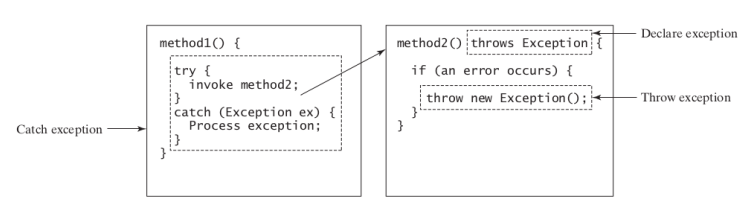
\includegraphics[scale=0.5]{imagenes/excepciones1.png}
\end{figure}
\end{frame}


\begin{frame}[fragile]
\frametitle{Ejemplo de excepeciones declarativas}
\begin{tiny}
\begin{verbatim}
import java.io.PrintWriter; 
import java.io.IOException; 

public class Main { 
    public static void main(String[] args) {         
        PrintWriter fichero; 
        try { 
            // Las siguientes dos líneas pueden lanzar una excepción de tipo IOException 
            fichero = new PrintWriter("ruta"); 
            fichero.write("Esto se escribirá en el fichero"); 
        } catch (IOException ioex) { 
            // Aquí capturamos cualquier excepción IOException que se lance (incluidas sus subclases) 
            ioex.printStackTrace(); 
        } 
         
    } 
}
\end{verbatim}
\pause
\begin{verbatim}
import java.io.PrintWriter; 
import java.io.IOException; 

public class Main { 
    // En lugar de capturar una posible excepción, la relanzamos 
    public static void main(String[] args) throws IOException {         
        PrintWriter fichero = new PrintWriter("ruta"); 
        fichero.write("Esto se escribirá en el fichero");     
    } 
}
\end{verbatim}
\end{tiny}
\end{frame}

\begin{frame}
\frametitle{Relanzar la excepción}
\begin{footnotesize}
\begin{itemize}[<+->]
\item En caso de querer relanzar la excepción, debemos declarar dicha intención en el final del método que contiene las sentencias que lanzan la excepción.
\item Lo hacemos mediante la claúsula \alert{throws}.
\item Hay que tener presente que cuando se relanza una excepción estamos forzando a nuestro método a capturarla o relanzarla.
\item Una excepción que sea relanzada una y otra vez hacia arriba terminará llegando al método primigenio.
\item En caso de no ser capturada por éste, producirá la finalización de su hilo de ejecución (thread).
\item La dos preguntas que debemos hacernos en este momento es: ¿Cuándo capturar una excepción? ¿Cuándo relanzarla?
\item Capturamos una excepción cuando:
\begin{enumerate}
\item Podemos recuperarnos del error y continuar con la ejecución.
\item Queremos registrar el error.
\item Queremos relanzar el error con un tipo de excepción distinto.
\item En definitiva, cuando tenemos que realizar algún tratamiento del propio error. 
\end{enumerate}
\item Por contra, relanzamos una excepción cuando no es competencia nuestra ningún tratamiento de ningún tipo sobre el error que se ha producido.
\end{itemize}
\end{footnotesize}
\end{frame}


\begin{frame}
\frametitle{Terminación o reanudación}
\begin{itemize}[<+->]
\item Hay dos modelos básicos en el manejo de excepciones: \emph{terminación o reanudación}.
\item En la \emph{terminación} se asume que el error es tan crítico que no hay forma de volver atrás a resolver dónde se dio la excepción.
\item En la \emph{reanudación} espera que el manejador haga algo para resolver la situación.
\item Una forma es usar un bloque \emph{while} que contiene el bloque \emph{try} que sigue intentando entrar en el bloque try hasta que se obtiene el resultado satisfactorio.
\end{itemize}
\end{frame}

\begin{frame}[fragile]
\frametitle{Creando excepciones propias}
\begin{footnotesize}
\begin{verbatim}
class ExcepcionSencilla extends Exception
{
}
public class DemoExcepcionSencilla
{
  public void metodo () throws ExcepcionSencilla
  {
    System.out.println ("Lanzando excepción desde metodo");
    throw new ExcepcionSencilla ();
  }
  public static void main (String[]arg)
  {
    DemoExcepcionSencilla s = new DemoExcepcionSencilla ();
      try
    {
      s.metodo ();
    } catch (ExcepcionSencilla e)
    {
      System.err.println ("Capturada excepción");
    }
  }
}
\end{verbatim}
\end{footnotesize}
\end{frame}



\begin{frame}[fragile]
\frametitle{Creando excepciones propias}
\begin{scriptsize}
\begin{verbatim}
class ExcepcionSencilla1 extends Exception
{
  public ExcepcionSencilla1 (String mensaje)
  {
    super (mensaje);
  }
}
public class OtraExcepcionSencilla
{
  public void metodo () throws ExcepcionSencilla1
  {
    System.out.println ("Lanzando excepción desde metodo");
    throw new ExcepcionSencilla1 ("originada en el metodo");
  }
  public static void main (String[]arg)
  {
    OtraExcepcionSencilla s = new OtraExcepcionSencilla ();
      try
    {
      s.metodo ();
    } catch (ExcepcionSencilla1 e)
    {
      e.printStackTrace (System.err);
    }
  }
}
\end{verbatim}
\end{scriptsize}
\end{frame}

\begin{frame}[fragile]
\frametitle{Creando nuestras propias excepciones}
\begin{scriptsize}
\begin{verbatim}
class ServerTimeOutException extends Exception {}

public void conectame( String nombreServidor ) throws Exception {
    int exito;
    int puerto = 80;
    
    exito = open( nombreServidor,puerto );
    if( exito == -1 )
        throw ServerTimeOutException;
}
\end{verbatim}
\pause
\begin{verbatim}
public void encuentraServidor() {
   ...
   try {
        conectame( servidorDefecto );
        } catch( ServerTimeOutException e ) {
          g.drawString( 
              "Time-out del Servidor, intentando alternativa",5,5 );
              conectame( servidorAlterno );
            }
    ...
}
\end{verbatim}
\end{scriptsize}
\end{frame}

\begin{frame}[fragile]
\frametitle{Creando excepciones propias}
\begin{itemize}[<+->]
\item El programador puede lanzar sus propias excepciones
\item Debemos usar la sintáxis \emph{extends Exception}
\end{itemize}
\end{frame}

\begin{frame}[fragile]
\frametitle{Ejemplo}
\begin{scriptsize}

\begin{verbatim}
public class TestTrianguloRectangulo {
   public static void main(String[] ar) throws NoTrianguloRectanguloException {
      TrianguloRectangulo t1 = new TrianguloRectangulo(1, 1, 2);
      TrianguloRectangulo t2 = new TrianguloRectangulo(1, 2, 5);
   }
}

class TrianguloRectangulo{
    private double cateto1;
    private double cateto2;
    private double hipotenusa;
    public TrianguloRectangulo(double cateto1,
           double cateto2, double hipotenusa) throws
    NoTrianguloRectanguloException{
        if (Math.pow(cateto1,2)+Math.pow(cateto2,2)==
            Math.pow(hipotenusa,2)){
            this.cateto1=cateto1;
            this.cateto2=cateto2;
            this.hipotenusa=hipotenusa;
        }
        else
            throw new NoTrianguloRectanguloException();
    }
}
\end{verbatim}

\end{scriptsize}
\end{frame}


\begin{frame}
\frametitle{Especificación de excepciones}
\begin{itemize}[<+->]
\item Para conocer como funciona un método, consultamos las especificaciones del mismo.
\item En ella nos informa del valor devuelto y el número y tipo de parámetros.
\item Pero también las excepciones que se deben lanzar.
\item La especificación de excepciones utiliza la palabra reservada \alert{throws}
\item De manera que la definicion del método puede quedar:
\end{itemize}
\pause
\begin{quote}
void f(\dots) \textbf{throws} Excepcion1, Excepcion2, \dots
\end{quote}
\end{frame}




\begin{frame}[fragile]
\frametitle{Capturar cualquier excepcion}
Esposible crear un manejador que capture cualquier tipo de excepcion:
\begin{verbatim}
catch(Exception e){
     ......
}
\end{verbatim}
\begin{itemize}[<+->]
\item Captura cualquier tipo de excepción, habrá que ponerla al \textbf{final del código de manejadores} para evitar que interfiera con alguno mas específico.
\item Ya que la clase \emph{Exception} es la base de todas.
\item Ademas se puede llamar a los métodos, para cualquier excepción, los derivados de la clase padre \alert{Throwable}
\begin{enumerate}
\item \alert{String getMessage()} información del mensaje.
\item \alert{String getLocalizedMessage()} información del mensaje.
\item \alert{String toString()} breve descripción del objeto \emph{Throwable}
\item \alert{void printStackTrace(), void printStackTrace(PrintStream), void printStackTrace(PrintWriter)} que imprime el obtejo y la traza de pila de llamadas lanzada.
\end{enumerate}
\end{itemize}
\end{frame}

\begin{frame}[fragile]
\frametitle{Ejemplo}
\begin{small}
\begin{verbatim}
public class MetodosExcepcion
{
  public static void main (String[]arg)
  {
    try
    {
      throw new Exception ("Aquí está la excepción");
    } catch (Exception e)
    {
      System.err.println ("Excepción capturada");
      System.err.println ("e.getMessage(): " + e.getMessage ());
      System.err.println ("e.getLocalizedMessage(): " +
                          e.getLocalizedMessage ());
      System.err.println ("e.toString(): " + e.toString ());
      System.err.println ("e.printStackTrace(): ");
      e.printStackTrace ();
    }
  }
}
\end{verbatim}
\end{small}
\end{frame}





\begin{frame}[fragile]
\frametitle{Clausula finally}
\begin{small}
\begin{itemize}[<+->]
\item A veces interesa lanzar un trozo de código independientemente que se lancen o no excepciones dentro de un bloque try.
\item Generalmente son operaciones relacionadas con recuperación de memoria.
\item Para esto se usa la clausula \alert{finally}
\item En Java el recolector de basura se encarga la liberacion de objetos no referenciados, por lo que la liberacion de memoria no es problema.
\item Pero \emph{finally} es muy recomendado para cerrar los flujos de I/O
\end{itemize}
\pause
\begin{verbatim}
try{
    actividades peligrosas A y B
}catch(A a1){
    manejador de la situación de A
}catch(B b1){
    manejador de la situación de B
}finally{
    actividades que se van a realizar
}
\end{verbatim}
\end{small}
\end{frame}

\begin{frame}[fragile]
\frametitle{Ejemplo finally}
\begin{scriptsize}
\begin{verbatim}
class Excepcion extends Exception{}
public class EjemploFinally{
  static int contador = 0;
  public static void main (String[]arg){
    while (true)
      {
        try
        {
          if (contador++ == 0)
            throw new Excepcion ();
            System.out.println ("Sin excepción");
        }
        catch (Excepcion e)
        {
          System.err.println ("Excepción");
        }
        finally
        {
          System.err.println ("Inicio de clausula finally");
          if (contador == 2)
            break;
        }
      }
  }
}
\end{verbatim}
\end{scriptsize}
\end{frame}

\begin{frame}[fragile]
\frametitle{Otro ejemplo de finally}
\begin{scriptsize}
\begin{verbatim}
public class FinallyDemo{
  public static void main (String[]args)
  {
    java.io.PrintWriter output = null;
    try
    {
// Crea un fichero
      output = new java.io.PrintWriter ("text.txt");
// Escribe en el fichero
      output.println ("Welcome to Java");
    }
    catch (java.io.IOException ex)
    {
      ex.printStackTrace ();
    }
    finally
    {
// Cierra el fichero
      if (output != null)
        output.close ();
    }
    System.out.println ("Fin del programa");
  }
}
\end{verbatim}
\end{scriptsize}
\end{frame}

\begin{frame}[fragile]
\frametitle{try-catch en Java SE 7}
\begin{verbatim}
public static void main(String[] args)
{
   try (BufferedReader reader = new BufferedReader(
   	new InputStreamReader(
   	new URL("http://www.yoursimpledate.server/")
   	   .openStream())))
   {
   	String line = reader.readLine();
   	SimpleDateFormat format = 
   	    new SimpleDateFormat("MM/DD/YY");
   	Date date = format.parse(line);
   } catch (ParseException | IOException exception) {
   	// handle I/O problems.
   }
}
\end{verbatim}
\uncover{No hace falta un bloque finally para cerrar los flujos abiertos, se cierran solos}
\end{frame}


\begin{frame}[fragile]
\frametitle{Malas practicas en el tratamiento de excepciones I}
\begin{scriptsize}
\begin{verbatim}
try { 
    // Código que declara lanzar excepciónes 
} catch(Exception ex) {}
\end{verbatim}
\end{scriptsize}
\pause
\begin{itemize}[<+->]
\item El código anterior ignorará cualquier excepción que se lance dentro del bloque try
\item Capturará toda excepción lanzada dentro del bloque try pero la silenciará no haciendo nada.
\item Cualquier error de diseño, de programación o de funcionamiento en esas lineas de código pasará inadvertido tanto para el programador como para el usuario. 
\item  Algo más razonable sería pintar una traza completa del error mediante uno de los métodos informativos de Throwable: 
\end{itemize}
\pause
\begin{scriptsize}
\begin{verbatim}
try { 
    // Código que declara lanzar excepciones 
} catch(Excepcion ex) { 
    ex.printStackTrace();    // Podemos añadir cualquier 
    tratamiento adicional antes y/o después de esta línea 
}
\end{verbatim}
\end{scriptsize}
\end{frame}

\begin{frame}[fragile]
\frametitle{Malas practicas en el tratamiento de excepciones II}
Otro abuso del mecanismo de tratamiento de excepciones es cuando se está intentando escribir código que mejore el rendimiento de la aplicación:
\begin{scriptsize}
\begin{verbatim}
try { 
    int i = 0; 
    while(true) { 
        System.out.println(numerosPrimos[i++]); 
    } 
} catch(ArrayIndexOutOfBoundsException ex) {}
\end{verbatim}
\end{scriptsize}
\pause
\begin{itemize}[<+->]
\item El ejemplo anterior itera sin preocuparse de los límites del array
\item Cuando se alcanza el índice máximo, momento en el cual se lanzará una excepción de tipo ArrayIndexOutOfBoundsException que será capturada y silenciada.
\item El tratamiento de excepciones está diseñado para gestionar excepciones y no para realizar optimizaciones 
\item  El resultado es estéticamente horrible.
\end{itemize}
\end{frame}

\begin{frame}[fragile]
\frametitle{Malas practicas en el tratamiento de excepciones III}
Otro error común se produce cuando estamos creando nuestra propia librería de excepciones y nos excedemos declarando excepciones checked:
\begin{scriptsize}
\begin{verbatim}
try { 
    // Código que declara lanzar muchas excepciónes 
} catch(UnTipoDeException ex1) { 
    // Gestionar... 
} catch(OtroTipoDeException ex2) { 
    // Gestionar... 
} catch(OtroTipoMasDeException ex3) { 
    // Gestionar... 
} catch(OtroTipoTodaviaMasDeException ex3) { 
    // Gestionar... 
}
\end{verbatim}
\end{scriptsize}
\end{frame}

\begin{frame}[fragile]
\frametitle{Malas practicas en el tratamiento de excepciones IV}
\begin{scriptsize}
\begin{verbatim}
public void miMetodo() throws Exception { 
    // Código que declara lanzar muchas excepciones. 
    // Sin embargo, en la firma del método declaramos
     lanzar una única super-clase de todas éllas 
}
\end{verbatim}
\end{scriptsize}
Los clientes de tu método no sabrán jamás con que condiciones especiales se pueden encontrar, y por tanto no podrán gestionarlas;
\end{frame}

\begin{frame}[fragile]
\frametitle{Malas practicas en el tratamiento de excepciones V}
\begin{itemize}[<+->]
\item Debemos pensar detenidamente si la excepción es de tipo checked o unchecked.
\item Cualquier situación excepcional que deje la aplicación en un estado irrecuperable y/o no sea inherente al proposito del código que la produce debe ser declarada como una excepción de tipo unchecked.
\item Existe una técnica para convertir toda excepción checked en unchecked:
\end{itemize}
\begin{scriptsize}
\begin{verbatim}
public void noLanzoExcepcionesChecked() { 
    try { 
        // Código que lanza una o más excepciones de tipo checked 
    } catch(Exception ex) { 
        throw new RuntimeException("Se ha producido una excepción con el
         mensaje: " + ex.getMessage(), ex); 
    } 
}
\end{verbatim}
\end{scriptsize}
\end{frame}

\begin{frame}[fragile]
\frametitle{Recomendaciones de uso}
\begin{itemize}[<+->]
\item Un buen uso del tratamiento de excepciones es usar excepciones que ya existen.
\item Se suelen usar excepciones que ya existen cuando se dispone de un profundo conociento del API que se está usando. (Mirar el API de la clase que se usa).
\item Si un argumento pasado a uno de tus métodos no es del tipo esperado, o no tiene el formato correcto, lanza una excepción IllegalArgumentException en lugar de crear tu propia excepción.
\item Documentar adecuadamente las excepciones que lanza el código.
\item Ejemplo:
\end{itemize}
\pause
\begin{tiny}
\begin{verbatim}
                /** 
                * @author Pepito  
                * @throws MiExcepcion se lanza en caso de ... 
                */ 
                public class MiClase throws MiExcepcion { 
                // ... 
                }
\end{verbatim}
\end{tiny}
\end{frame}

\begin{frame}
\frametitle{Miscelánea}
\framesubtitle{Clase ResourceBundle}
\begin{itemize}[<+->]
\item Un fichero de propiedades es un simple fichero de texto que se puede crear y mantener con un sencillo editor de texto. 
\item Cada línea define una propiedad y su correspondiente valor.
\item El nombre de este fichero empieza por el nombre base y termina con el sufijo \emph{.properties}.
\item Se suele usar para la internacionalización de las aplicaciones.
\item Ejemplo usuario.properties:
\end{itemize}
\pause
\begin{quote}
username=manuel\\
password=pppd!we\\
nombre=Manuel Garcia\\
email=mgarcia@iesvirgendelcarmen.com
\end{quote}
\end{frame}

\begin{frame}[fragile]
\frametitle{Ejemplo}
\begin{tiny}
\begin{verbatim}
import java.util.ResourceBundle;
public class Aplicacion
{
  public Usuario login (String usrname, String pass)
  {
    try
    {
      ResourceBundle rb = ResourceBundle.getBundle ("usuario");
      String usr = rb.getString ("username");
      String pas = rb.getString ("password");
      Usuario u = null;
      if (usr.equals (usrname) && pas.equals (pass))
        {
          u = new Usuario ();
          u.setUsername (usr);
          u.setPassword (pas);
          u.setNombre (rb.getString ("nombre"));
          u.setEmail (rb.getString ("email"));
        }
      return u;
    }
    catch (Exception ex)
    {
      throw new RuntimeException ("Error verificando datos", ex);
    }
  }
}
\end{verbatim}
\end{tiny}
\end{frame}

\begin{frame}
\frametitle{FIN}
\begin{figure}

\includegraphics[scale=0.4]{imagenes/end.png}
\end{figure}
\end{frame}

\end{document}